\section{Previous approaches}
\label{sec:approaches}

If the above foray into the threat models concerning language generation that have been discussed in research has revealed anything, it is that expecting model operators to disclose the nature of texts submitted to their recipients is a naive and potentially dangerous habit.
Thankfully, as language models have grown larger and more sophisticated, so have strategies and technologies detecting them matured alongside them.
Though it has certainly received and influx of manpower interest since then, the field of automatic detection of machine generated text has been an active area of research even from before 2020 -- after all, as was previously discussed, there was no shortage of attempts to exploit NLG technologies well before the recent GPT craze.

In Chapter \ref{sec:background}, this thesis presented an overview of different ways in which text could be represented, on a spectrum ranging from surface-level metrics to neural contextual embeddings.
Many parallels can be drawn between these strategies and the methodologies employed to detect machine generation.
In the following sections, several well researched and empirically tested detection strategies will be explored, some taking advantage of linguistically motivated features or even frequency-based metrics, while others lean into the times and use LLMs themselves to discriminate between authentic and generated productions.
It should however be underlined that the movement toward more sophisticated vectorization processes does not necessarily entail a one-sided improvement across all possible aspects involved in the detection pipeline.

On the contrary, moving up the ladder of complexity comes at the cost of requiring increasing amounts of computational power.
Such approaches are extremely valid explorations of what is the best that can be achieved, but applicability in the real world is often limited since the end users cannot run the required software on commonplace commercial machines.
Separating the application into client and server, which is the common approach taken in other AI fields, is only acceptable in the narrower subset of cases which have no privacy requirement regarding the data being verified.
Chapter \ref{sec:task} will dive deeper into the more "cheap" approaches, meaning those that forgo heavy systems, aiming instead to strike a balance between performance and (compute) accessibility.

\subsection{Frequency and feature-based methods}

A simple way to think of documents is as so-called bags of words (BOW) \citep{murphy2006naive}.
BOW representation strategies only consider the words that appear in a text, without maintaining any information about the order.
One application is the simple count vectorization strategy \citep{wendland2021introduction}, in which a text is represented by the counts of each word that occurs in it.

A closely related, but more refined and widely applied method is the extraction of TF-IDF matrices over sets of documents \citep{ramos2003using}.
If one only looks at word counts, then prepositions and other common elements will likely account for much of the information retrieved from the text.
TF-IDF offers a fix by implementing the intuition that a text containing the words "geothermal" and "power-plant", even if only with a few occurrences, is more informative about its nature than it having hundreds of examples "the" and "of".
As such, term frequencies in TF-IDF are weighted by how rare they are (i.e. in how many documents of the sample they appear), with rarer words gaining a proportional score boost.

TF-IDF has a rich history of successful usage in almost all fields of NLP, including information retrieval \citep{ramos2003using}, sentiment analysis \citep{cahyani2021performance}, and text-classification \citep{zhang2011comparative} among many others.
Machine text detection has also tapped into this tradition.
Recently, \citet{frohling2021feature} employed higher-dimensional TF-IDF both as a classification accuracy baseline and as an input to meta-learners, i.e. ensemble models that take predictions from multiple classifiers to produce a final label.
While falling short of state-of-the-art solutions that will be discussed later in this chapter, this methodical experiment still managed to build competitive systems by combining (computationally) simple approaches, in part by drawing upon the information captured by TF-IDF.

Alongside n-gram frequency features, like the ones discussed so far, another common approach to text vectorization is represented by linguistic feature sets.
Instead of relying on simple token counts to derive a way to represent human productions with numbers, this strategy utilizes the quantifiable properties of the language being used.
Some trivial examples may be the global length of a text, the average word length of the sentences contained within it, the type-token ratio, and so forth.
Naturally, one can devise much more refined metrics to extract from texts, for example regarding text fluency, readability, grammatical properties, the richness of the vocabulary, cohesion, or even its purpose.
The inquiry mentioned above, conducted by \citet{frohling2021feature}, combined TF-IDF representations with feature-based classifiers across a variety of settings and datasets -- in fact, these linguistic features drive most of the best models' performance.

The first targetable linguistic characteristic that language models have been observed to exhibit is a lack of cohesion \citep{holtzman2019curious}.
A study on GPT-2, for example, found that decoding strategies that maximize overall probability are likely to run into repetitive language \citep{see2019massively}, and even topic-drift, a phenomenon in which language models fail to stay within the confines of a particular topic \citep{badaskar2008identifying}.
Traditional readability features, such as the Gunning-Fog Index and the Flesch-Kincaid Index, have been used successfully to identify generated text \citep{Crothers_2022}.
Other methods involve modeling relationships between entities across documents through auxiliary models \citep{barzilay2008modeling}, which seek to automatically determine the primary elements of the text, and track how they are presented throughout a text -- with the idea being that human authors will refer back to the main points more often than machines.

Another useful set of features involve the use of varied vocabulary, and one that avoids repetition as much as possible.
Texts authored by humans typically exhibit creative strategies to maintain narrative flow, such as building deep coreference chains instead of bogging down the text with frequent repetitions \citep{feng2010comparison} -- LMs tend instead to err toward toward the opposite side \citep{gehrmann2019gltrstatisticaldetectionvisualization}.
Generated text display frequent use of repetition, leading to reduced lexical diversity within the text \citep{zellers2020evaluating}.
Lexical richness is, fortunately, one of the language aspects that can be more readily measured through features such as type-token ration, content or stop-word ratio, POS-tag distribution, and frequency of rare words, among many \citep{van2007comparing}.
\citet{see2019massively} identify a concrete trend in word-type usage in generated texts, where LMs favor verbs and pronouns more than humans, who make richer use of nouns and adjectives.
Moreover, the reduced usage of varied ways to refer to entities can be measured by extracting the length of coreference chains \citep{feng2010comparison}, with the expectation that machines will produce shorter chains and more explicit repetitions.

The repetitive nature of generated text can also be attributed to the underlying sampling strategies.
\citet{ippolito2019automatic} observe that a huge proportion of the probability mass is concentrated in the first few hundred, most common tokens in the case of top-k sampling.
To make use of this property, another set of features measuring frequency of common texts can be employed, and it can lead to good detection performance when the model is sampled with top-k (other sampling methods do not necessarily exhibit the same tendency).

Typically, generated text detection is a supervised task, which means that model training takes place with a labelled set of data.
One interesting study explores the issue at hand with an unsupervised strategy: \citet{galle2021unsupervised} use repeated high-order n-grams (re-occurring multi-word expressions) to distinguish machine text from human productions.
They find that \emph{supermaximal} substrings (i.e. the longest substrings that do not occur in any other substring of the collection) can be efficiently computed for a collection, and their presence in texts can be used as input for binary prediction.
Specifically, they randomly select a subset of supermaximal repeats, and pre-label every document containing them as machine-generated. Then, these are used as positive examples to train a classifier, with an equal number of human texts as negative examples (they experiment with separate true human texts, as well as presumably human, picked at random from the same unannotated collection).
This process is repeated a number of times with different selections of repeated substrings, and the results from each classifier is combined into a final ranking.
The result is a list, where the top-scoring items are highly suspected to be machine-generated.
Precision is then reported regarding the top \emph{m} documents in the ranking, since the authors' intent is to design a system that pushes the final decision onto human judges, with the intent of only identifying suspicious documents.
As summarized in Figure \ref{fig:galle2021_fig5_100models}, this approach was tested against GPT-2 and it was able to reach an impressive 80\% precision (in top-5000) even with nucleus sampling \citep{holtzman2019curious}, which makes generation much harder to detect than top-k strategies (which this strategy detects at near-perfect precision) and is therefore an extremely interesting strategy when only few in-domain examples are available.

\begin{figure}[h]
    \centering
    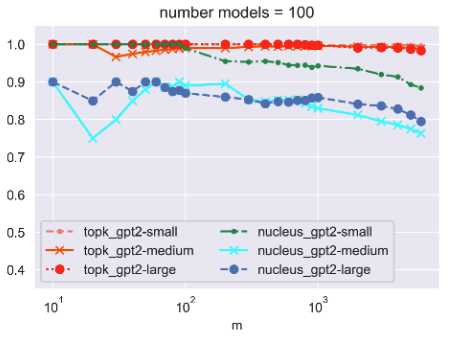
\includegraphics[width=0.6\textwidth]{assets/galle2021_fig5_100models.png}
    \caption{
        Precision reported by \citet{galle2021unsupervised} for most suspicious documents, with 100 separate classifiers informing the decision.
        \emph{m} indicates the precision at the first \emph{m} elements of the ranking.
        It is noteworthy that precision for GPT2-Large with nucleus sampling stays relatively high even at \emph{m} in the thousands.
    }
    \label{fig:galle2021_fig5_100models}
\end{figure}

\subsection{Neural approaches}

The strategies discussed so far have been traditionally paired been used with statistical models (chiefly logistic regression and support vector machines).
However, the field of generated text detection has naturally also adopted the huge technological shift which of NLP has experienced, represented by neural networks and neural language models \citep{papers2024nlp}.
Since statistical features predictably underperform neural features \citep{crothers2022adversarial}, most detection approaches in this area forgo linguistic and frequency-based features altogether.
However, recent results confirm their validity even when employed alongside LLMs: although they reach lower peaks than transformer-based counterparts, they are much more robust against adversarial attacks.
Adversarial attacks describes malicious attempts of various types made by third parties to induce a misclassification in the model.
Some examples may be illicitly accessing the training data of the detector model and insert or corrupt its records, or intercept the input at inference time and introduce changes in order to evade detection.
In this context, an attacker might introduce small perturbations (like word or character edits) into the generated text to make the detector model fail to notice the generation.
Statistical features were observed to have very high resistance to such attacks, and a hybrid model combining statistical features with Transformer-based attributes was reported to significantly enhance adversarial robustness, while maintaining solid performance in standard, non-adversarial scenarios \citep{crothers2022adversarial}.

Of course, no survey into the various methods to detect automatic generation can ignore the two classes of state-of-the-art approaches, both rooted in leveraging pretrained neural language models.
On one side, there are so-called zero-shot approaches \citep{zellers2020defendingneuralfakenews}, which take advantage of the logits outputted by the models and attempt to make a prediction based on those, with various degrees of sophistication.
On the other, approaches based on fine-tuning large bi-directional transformers \citep{solaiman2019release} boast the contribution of the absolute best models to the field at present.
The BERT variant RoBERTa \citep{liu2019robertarobustlyoptimizedbert} has emerged as a winner in this space, both because due to its strong performance, as well as the relative ease with which fine-tuning approaches can be taken off the ground \citep{radford2019dataset}.

A comprehensive research suite conducted by \citet{zellers2020defendingneuralfakenews} has evaluated GPT-2 and GROVER (a transformer LM geared towards article generation which they themselves introduced) in an effort to use them as discriminators for machine-generated text.
Following \citep{radford2018improving}, this study runs the input texts through the models with a special \emph{[CLS]} token in the final position.
The output embeddings corresponding to this token are then passed onto a linear layer performing binary classification.
Evaluation then proceeds for different model sizes both for the generator (GROVER is also used to generate the articles to be predicted) and the discriminator.
Perhaps unsurprisingly, the GROVER-based discriminators are best at detecting the GROVER-generated AI texts, and detection accuracy decreases as the generator is allowed more parameters (but classifiers benefit from positive examples generated by smaller models even against the largest model's outputs).
Unfortunately, as is often the case in even very recent research, newer GPT variants are prohibitively expensive \citep{galle2021unsupervised} to employ on large benchmark datasets, which leads to few front-runner studies reporting results with them.

To date, DetectGPT \citep{mitchell2023detectgptzeroshotmachinegeneratedtext} is the best zero-shot approach to detect generated text, and the best detection tool for out-of-domain classification in general, at least in the white box setting \citep{gehrmann2019gltrstatisticaldetectionvisualization}.
This strategy leverages the observation that machine-generated text is much more susceptible to log probability perturbation (according to the source model) when edits are introduced to it, i.e. altering words or rewriting short passages of the text will cause the log probability to fall measurably.
On the contrary, human-written texts do not exhibit the same property, and their log probability may change in a variety of ways in response to perturbation, but edits that preserve the semantic meaning of the text will tend to cause no perturbation at all.
Armed with this knowledge, DetectGPT introduces minor, sense-preserving edits (such as swapping words for synonyms or rewriting pieces with mask-filling) to a target text through an auxiliary model -- in this study, T5 \citep{raffel2023exploringlimitstransferlearning} -- end evaluates the difference in log probability between the original and altered versions.
If the difference is above a certain threshold, the input is flagged as machine-generated.

DetectGPT outperforms even RoBERTa-based models when the target text is outside of the domain of the fine-tuned transformers' training sets, while still maintaining near-top performance when in-distributed texts are classifier.
The simpler task definition of the white box setting, i.e. that the generator model is known accessible, is however a limitation of the experiment.
Real-world scenarios can often include situations in which the generator model is unknown, therefore a proxy scorer needs to be used instead \citep{mireshghallah2023smaller}.
Figure \ref{fig:detectgpt} offers an overview of DetectGPT performance across different scoring and generator models.
Performance is predictably best when the scoring model is the same as the generator, but good-enough alternative models can be found -- perhaps smaller, efficient models can be found for detecting the prominent generators, contributing to a less resource-intensive solution landscape.
Ensemble solutions may even cover against many potential generators, instead of relying on a single scoring model in the black box setting (i.e. when the generator model is not known).

\begin{figure}[h]
    \centering
    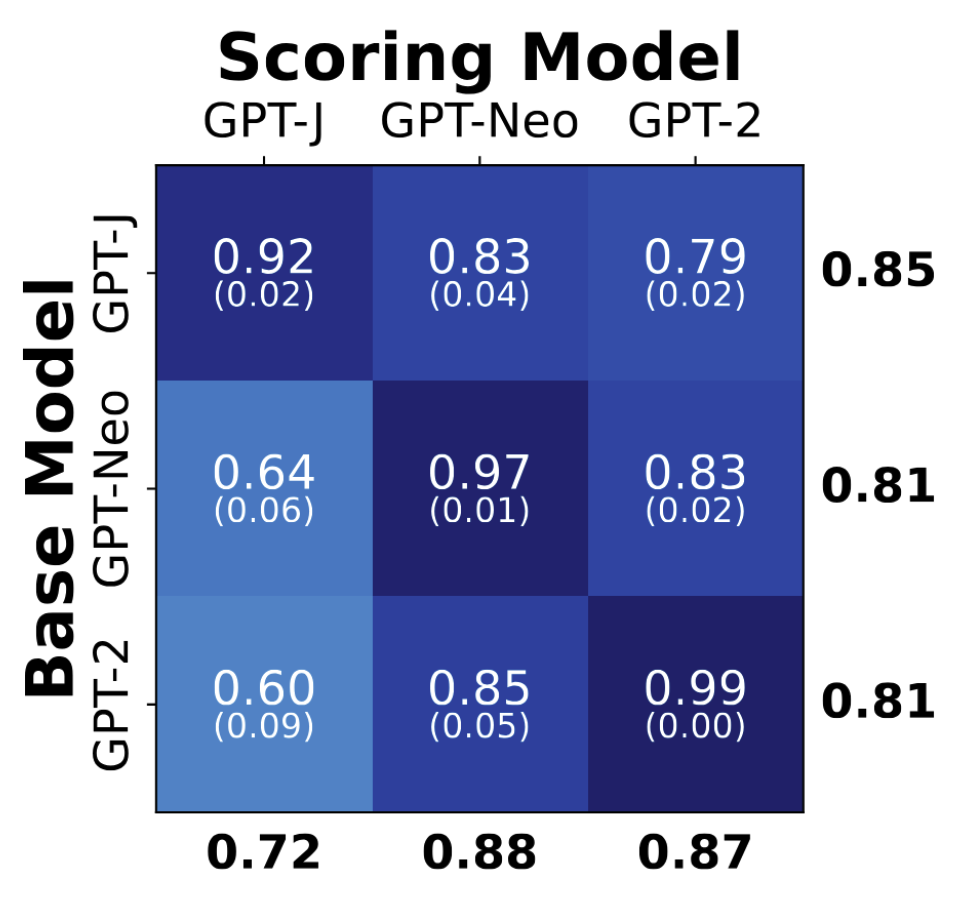
\includegraphics[width=0.5\textwidth]{assets/detectgpt_modelcomp.png}
    \caption{
        Performance overview of DetectGPT \citep{mitchell2023detectgptzeroshotmachinegeneratedtext}, reporting AUROC \citep{bradley1997use} over the XSum, SQuAD, and WritingPrompts datasets.
        Same scorer-generator pairs show the best performance, but results show that some models may act as better proxies than others, inviting further research.
    }
    \label{fig:detectgpt}
\end{figure}

The state-of-the art approach in machine-generated text detection has been, for a couple years at the time of writing, indisputably the fine-tuning approach \citep{solaiman2019release}.
This involves fine-tuning a pre-trained bi-directional language model.
The best resulting model is derived from providing task-specific training to RoBERTa \citep{liu2019roberta}, a masked general-purpose language model based on BERT \citep{devlin2019bertpretrainingdeepbidirectional} with a focus on classification.
The primary weakness of RoBERTa is that it doesn't necessarily handle cross-domain examples out of the box, an aspect that the aforementioned DetectGPT \citep{mitchell2023detectgpt} improved on greatly, despite not outgunning RoBERTa large from in-distribution datasets.
\citet{rodriguez2022cross} also offer an improvement on this front by evaluating model performance on a new domain with a few hundred attacker examples selected by experts.
While DetectGPT might be very useful in situations where the attacker characteristics are entirely unknown, this latter approach might still offer more in the more standard case of a back-and-forth effort between attackers and defenders.

\subsection{Domain differentiation}

Aside from general solutions mentioned above to the problem of generated text detection, there is a rich inventory of domain-specific tools and strategies.
For example, \citet{rodriguez2022cross} experiment with detection tasks in the technical domain, specific targeting physics and chemistry.
The study successfully applies a RoBERTa-based classifier fine-tuned on the biomedical domain on the physics domain, with relatively few new examples obtained from human experts.
While only relating to GPT-2, the results reported are encouraging in the sense that knowledge may be more easily transferable across similar domains, even if they are technical in nature.

In the real of social media, Twitter has received consistently high research attention.
\citet{fagni2021tweepfake} report on a number of different strategies that can help detect generated tweets, including some that are less commonly seen in research nowadays, such as TF-IDF and character-level models.
Interestingly, character-encodings outperformed BERT-based approaches, and only lagged 0.05 percentage points behind RoBERTa, further underlining the validity of imperfect but computationally realistic solutions.
\citet{tourille2022automatic} expand on this by introducing more training examples from GPT-2, which proved significantly harder to correctly classify in the original by \citet{fagni2021tweepfake}, and show that prediction accuracy can be boosted in this way, though globally this is hard to notice, since RoBERTa already had greater than 90\% accuracy.
In general, it is hard not to raise the criticism anew that all of the most recent research, including the aforementioned twitter studies, do not move beyond GPT-2, so it remains a question how well they would perform if the attacker models were the much more sophisticated contemporary LLMs.

Another interesting domain of detection is chatbots and direct messages.
Bot detection is already a well-researched field \citep{latah2020detection} where NLP can make a contribution when it comes to detecting AI agents faking human personhood.
\citet{bhatt2021detectingbotgeneratedtextcharacterizing} expand the methodologies applied here by analyzing not only the messages suspected of having been generating, but also how the human interlocutors reacted to them.
They verify the results with a number of different models across different representational strategies, such as BOW models, feature-based ones, and BERT-based classifiers.
Not only does the inclusion of the human responses into the input improve cross-dataset generalization of the models, but non-BERT models fall short of simpler BOW models for some (substantially different) cross-dataset runs.
Unfortunately, this experiments was again completed on the Conv2AI \citep{dinan2019secondconversationalintelligencechallenge} dataset, which does not make use of the most recent LLM technology in its generated examples.

Lastly, product reviews are also an area of interest when it comes to detecting automated text.
Recently, \citet{salminen2022creating} have used ULMFiT \citep{howard2018universal} and GPT-2 to generate fake reviews based on the Amazon \citep{ni2019justifying} dataset.
They then use this newly generated dataset to fine-tune a RoBERTa-based classifier, which they compare against an SVM model and an OpenAI off-the-shelf fake review detector, also a RoBERTa classifier.
Results show that the newly created model outperforms both baselines, reaching over 90\% accuracy.
These findings are validated against the Deceptive Reviews Dataset \citep{ott2011finding}, where the newly introduced classifier again obtains the best result of the three models, with an AUC of 0.696, followed by OpenAI's off-the-shelf model with 0.595.
Automated detection strategies seem especially necessary in this area, since the study also finds that human judges do not perform better than chance at identifying generations.
The adversarial nature of machine-generated text detection is especially at the forefront in this area, since it is easy to imagine a future in which attackers and detectors play a "cat-and-mouse" game, with attackers trying to evade detectors, and the latter developing new models and strategies in turn.
